\documentclass[10pt]{article}
\usepackage[utf8]{inputenc}
\usepackage[T1]{fontenc}
\usepackage[spanish]{babel}
\makeatletter\def\es@sppercent{}\makeatother
\usepackage{geometry}
\usepackage{multicol}
\usepackage{graphicx}
\usepackage{amsmath}
\usepackage{amssymb}
\usepackage{caption}
\usepackage{capt-of}
\usepackage{booktabs}
\usepackage{array}
\usepackage{times}
\usepackage{mathptmx}
\usepackage{titlesec}
\usepackage[hidelinks]{hyperref}
\usepackage{color}

\geometry{
    paper=letterpaper,
    top=0.98in,
    bottom=0.87in,
    left=0.59in,
    right=0.45in
}

\titleformat{\section}
  {\normalfont\bfseries\small}{\thesection.}{0.4em}{\MakeUppercase}
\titlespacing{\section}{0pt}{6pt}{2pt}

\titleformat{\subsection}
  {\normalfont\bfseries\small}{\thesubsection}{0.4em}{}
\titlespacing{\subsection}{0pt}{4pt}{1pt}

\setlength{\columnsep}{0.28in}
\setlength{\parindent}{0em}
\setlength{\parskip}{3.5pt}

% Spacing around captionof figures
\setlength{\intextsep}{4pt}
\setlength{\abovecaptionskip}{3pt}
\setlength{\belowcaptionskip}{2pt}

\captionsetup{font=small, labelfont=bf, justification=centering}

% Para insertar cada imagen: descomenta la línea \includegraphics y elimina el \vspace correspondiente

\pagestyle{empty}

% ──────────────────────────────────────────────
\begin{document}

%% ---- CABECERA ----
\begin{center}
{\large\bfseries
Magnetismo y Electromagnetismo: Visualización de Líneas de Campo, Ley de Ampere,\\
Corrientes de Foucault e Inducción Electromagnética}

\vspace{5pt}
{\normalsize Alexander Márquez Corzo}

\vspace{2pt}
{\small Departamento de Física \textbullet\ Universidad del Magdalena, Santa Marta}
\end{center}

\vspace{6pt}
\hrule height 0.8pt
\vspace{6pt}

%% ---- RESUMEN ----
\begin{center}{\small\bfseries Resumen}\end{center}
{\small
Se estudian cuatro fenómenos electromagnéticos fundamentales. En la primera mesa se visualizan las líneas de campo de un toroide, un solenoide y un imán cilíndrico usando limadura de hierro. En la segunda mesa se verifica la ley de Ampere con un sensor de campo magnético sobre tres trayectorias cerradas alrededor de un aro con corriente, obteniendo $\oint \vec{B}\cdot d\vec{l} \approx \mu_0 N I_{\text{enc}}$ con error del $8.4\,\%$ cuando la trayectoria encierra la corriente, y valores cercanos a cero en los demás casos. En la tercera mesa se estudian las corrientes de Foucault comparando el frenado de tres láminas de aluminio con distintas geometrías de ranuras. En la cuarta mesa se estudia el transformador y la ley de Faraday con bobinas intercambiables sobre núcleo de hierro, verificando $V_s/V_p = N_s/N_p$ y que la fem inducida depende del número de espiras y la velocidad de variación del flujo.}

\vspace{5pt}
\begin{center}{\small\bfseries Abstract}\end{center}
{\small
Four fundamental electromagnetic phenomena are studied experimentally. The first station visualizes the magnetic field lines of a toroid, a solenoid, and a cylindrical magnet using iron filings. The second station verifies Ampere's law by tracing three closed paths around a current-carrying loop with a wireless magnetic sensor, obtaining $\oint \vec{B}\cdot d\vec{l} \approx \mu_0 N I_{\text{enc}}$ with an $8.4\,\%$ error when the path encloses the current, and near-zero values otherwise. The third station demonstrates eddy-current braking with three aluminum plates of different slot geometries. The fourth station studies transformer principles and Faraday's law using interchangeable coils on an iron core, confirming $V_s/V_p = N_s/N_p$ and showing that the induced EMF depends on the number of turns and the rate of flux change.}

\vspace{6pt}
\hrule height 0.8pt
\vspace{5pt}

%% ============================================================
\begin{multicols}{2}
%% ============================================================

% -----------------------------------------------------------
\section{Introducción}
% -----------------------------------------------------------

El magnetismo y el electromagnetismo son dos de los temas más importantes de la física clásica. Desde una brújula hasta los transformadores que alimentan nuestras ciudades, los principios del campo magnético tienen aplicaciones en casi toda la tecnología eléctrica que usamos a diario.

En esta práctica se desarrollaron cuatro experimentos que permiten explorar de forma visual y cuantitativa los conceptos clave del electromagnetismo: la geometría de las líneas de campo, la ley de Ampere, las corrientes de Foucault y la inducción electromagnética aplicada al transformador.

La idea principal es que la física no se aprende solo con ecuaciones. Ver cómo la limadura de hierro dibuja las líneas de campo de un solenoide, o cómo una lámina de aluminio frena en seco al pasar junto a un imán, da una intuición que resulta muy difícil de transmitir únicamente con fórmulas.

% -----------------------------------------------------------
\section{Teoría Relacionada}
% -----------------------------------------------------------

\subsection*{Líneas de campo magnético}

El campo magnético $\vec{B}$ se representa mediante líneas de campo: curvas cuya tangente en cada punto indica la dirección del campo. A diferencia del campo eléctrico, estas líneas \emph{siempre son cerradas}, lo que significa que nunca comienzan ni terminan en un punto del espacio. Esto se expresa con la ley de Gauss para el magnetismo:
\begin{equation}
    \oint_S \vec{B}\cdot d\vec{A} = 0,
    \label{eq:gauss_mag}
\end{equation}
que nos dice que no existen monopolos magnéticos: todo imán tiene siempre un polo norte y un polo sur [1].

En un \textbf{solenoide} de $n$ espiras por unidad de longitud con corriente $I$, el campo interior es uniforme:
\begin{equation}
    B = \mu_0 n I,
\end{equation}
con $\mu_0 = 4\pi\times10^{-7}$~T·m/A. En un \textbf{toroide}, el campo queda completamente confinado dentro del núcleo y es nulo en el exterior [1].

\subsection*{Ley de Ampere}

La ley de Ampere dice que la integral del campo magnético a lo largo de cualquier camino cerrado es proporcional a la corriente que ese camino encierra:
\begin{equation}
    \oint_C \vec{B}\cdot d\vec{l} = \mu_0 \sum I_{\text{enc}}.
    \label{eq:ampere}
\end{equation}
Lo más importante de esta ley es que no depende de la forma del camino, sino de si ese camino ``encierra'' o no al conductor con corriente. Si el camino no pasa alrededor de ninguna corriente, la integral da cero, sin importar cómo sea el trayecto [2].

\subsection*{Corrientes de Foucault}

Cuando un conductor se mueve dentro de un campo magnético, la ley de Faraday hace que se induzcan en él corrientes circulares llamadas \emph{corrientes de Foucault}. Por la ley de Lenz, estas corrientes se oponen al movimiento, generando una fuerza de frenado.

Qué tan intensas sean estas corrientes depende de la geometría del conductor. En una placa \emph{sólida}, los electrones pueden circular en lazos grandes, lo que da corrientes grandes y mucho frenado. Si se le hacen \emph{ranuras}, esos caminos se interrumpen, las corrientes se reducen y el frenado disminuye [3]. Este principio es el que justifica que los núcleos de los transformadores se fabriquen con láminas delgadas apiladas: así se reducen las pérdidas por corrientes de Foucault.

\subsection*{Inducción y transformador}

La ley de Faraday establece que una fuerza electromotriz (fem) se induce en una bobina cuando el flujo magnético que la atraviesa varía:
\begin{equation}
    \mathcal{E} = -N\frac{d\Phi_B}{dt},
    \label{eq:faraday}
\end{equation}
donde $N$ es el número de espiras. A más espiras, mayor fem; y a mayor velocidad de cambio del flujo, también mayor fem [1].

El \textbf{transformador} usa este principio acoplando dos bobinas mediante un núcleo de hierro. La relación entre los voltajes es:
\begin{equation}
    \frac{V_s}{V_p} = \frac{N_s}{N_p},
    \label{eq:transformador}
\end{equation}
donde los subíndices $p$ y $s$ indican el devanado primario y secundario respectivamente. En la práctica la eficiencia no es del $100\,\%$ por pérdidas en el alambre, en el núcleo, y especialmente por la baja inductancia del primario cuando tiene pocas espiras [2].

% -----------------------------------------------------------
\section{Montaje y Procedimiento}
% -----------------------------------------------------------

\subsection*{Mesa 1: Visualización de líneas de campo}

Se conectaron un toroide y un solenoide de alambre de cobre a una fuente de corriente directa. Se roció limadura de hierro sobre cada uno y, al encender la fuente y dar pequeños golpes al soporte, las partículas se alinearon con las líneas de campo mostrando claramente su geometría. También había un imán cilíndrico dentro de una cápsula acrílica transparente rellena de limadura de hierro, que permitía ver las líneas en tres dimensiones.

\vspace{3pt}
\begin{center}
  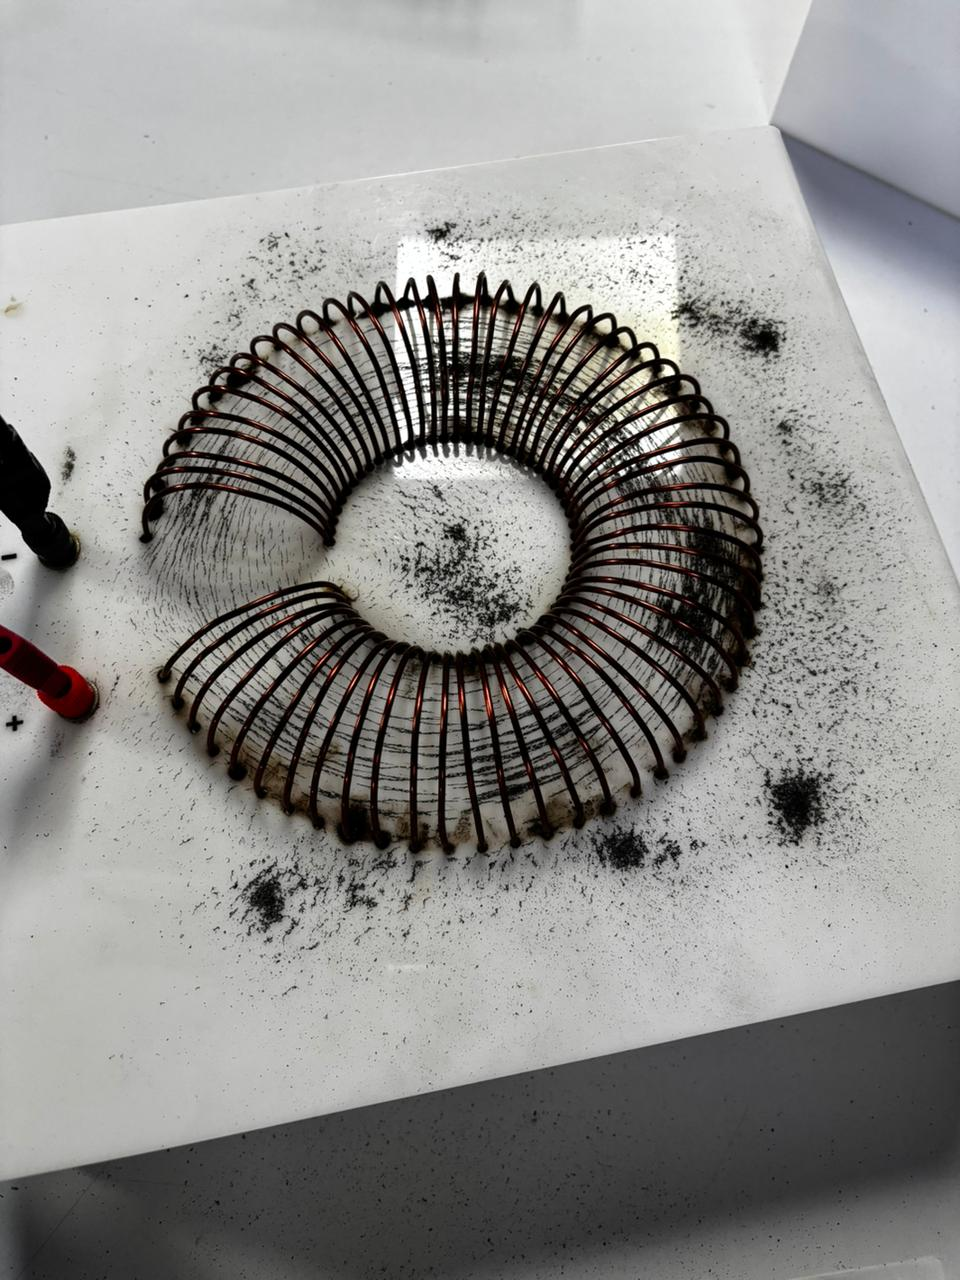
\includegraphics[width=\linewidth,height=5.5cm,keepaspectratio]{toroide.jpeg}
  \captionof{figure}{Toroide con limadura de hierro. Las líneas de campo quedan completamente confinadas dentro del núcleo toroidal, sin flujo en el exterior.\label{fig:toroide}}
\end{center}
\vspace{2pt}

\vspace{3pt}
\begin{center}
  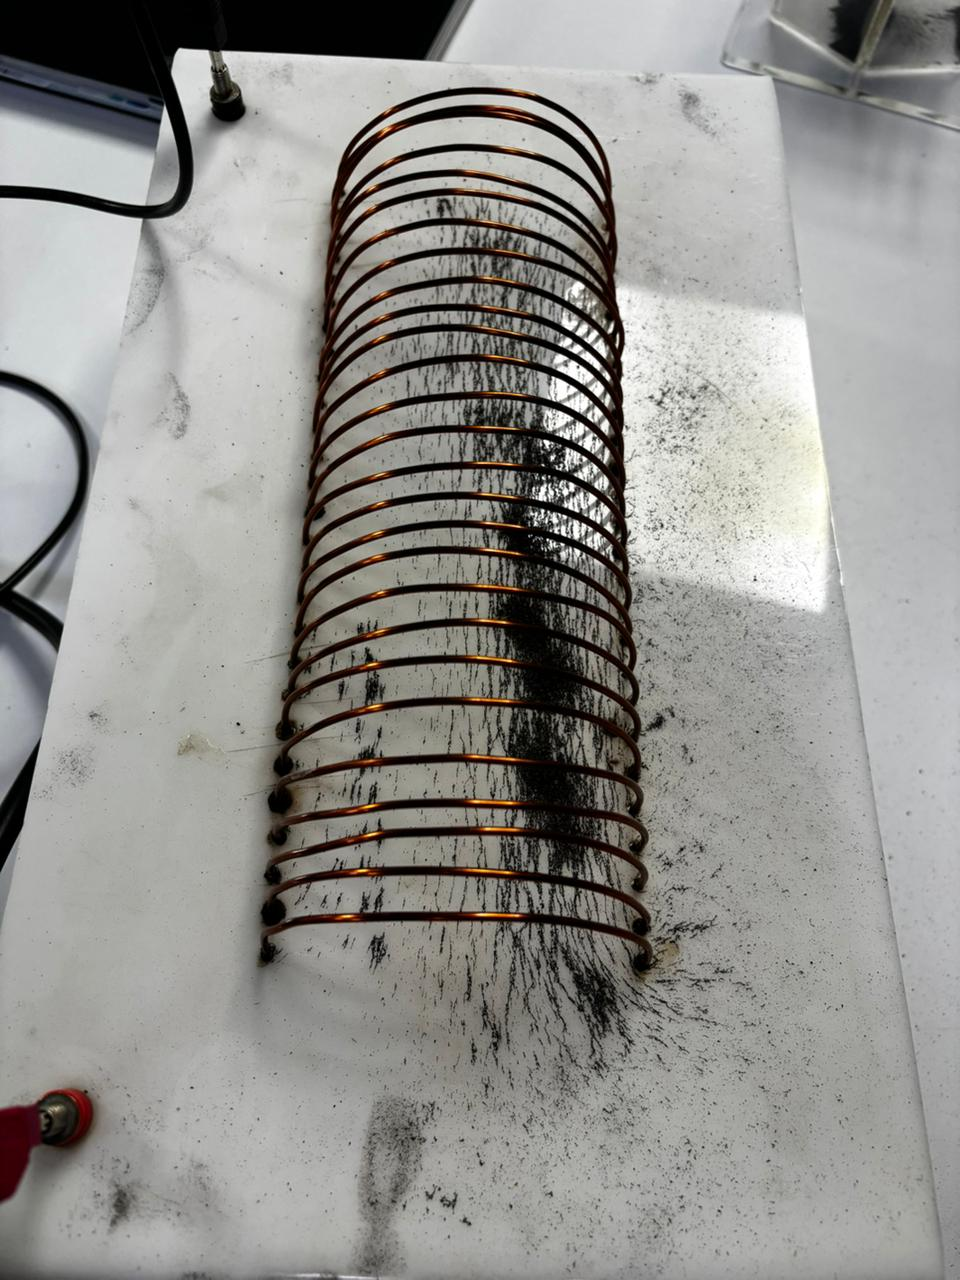
\includegraphics[width=\linewidth,height=5.5cm,keepaspectratio]{solenoide.jpeg}
  \captionof{figure}{Solenoide con limadura de hierro. Las líneas emergen por un extremo y se cierran por el otro, igual que en un imán de barra.\label{fig:solenoide}}
\end{center}
\vspace{2pt}

\subsection*{Mesa 2: Verificación de la ley de Ampere}

Se usó el aparato PASCO Ampere's Law (EM-6720): una plataforma con un aro conductor circular con corriente conocida, y un carro con sensor inalámbrico de campo magnético que se desplaza manualmente. El software PASCO Capstone registra $B_x$ en función de la posición y calcula la integral $\oint \vec{B}\cdot d\vec{l}$ como el área bajo esa curva.

\vspace{3pt}
\begin{center}
  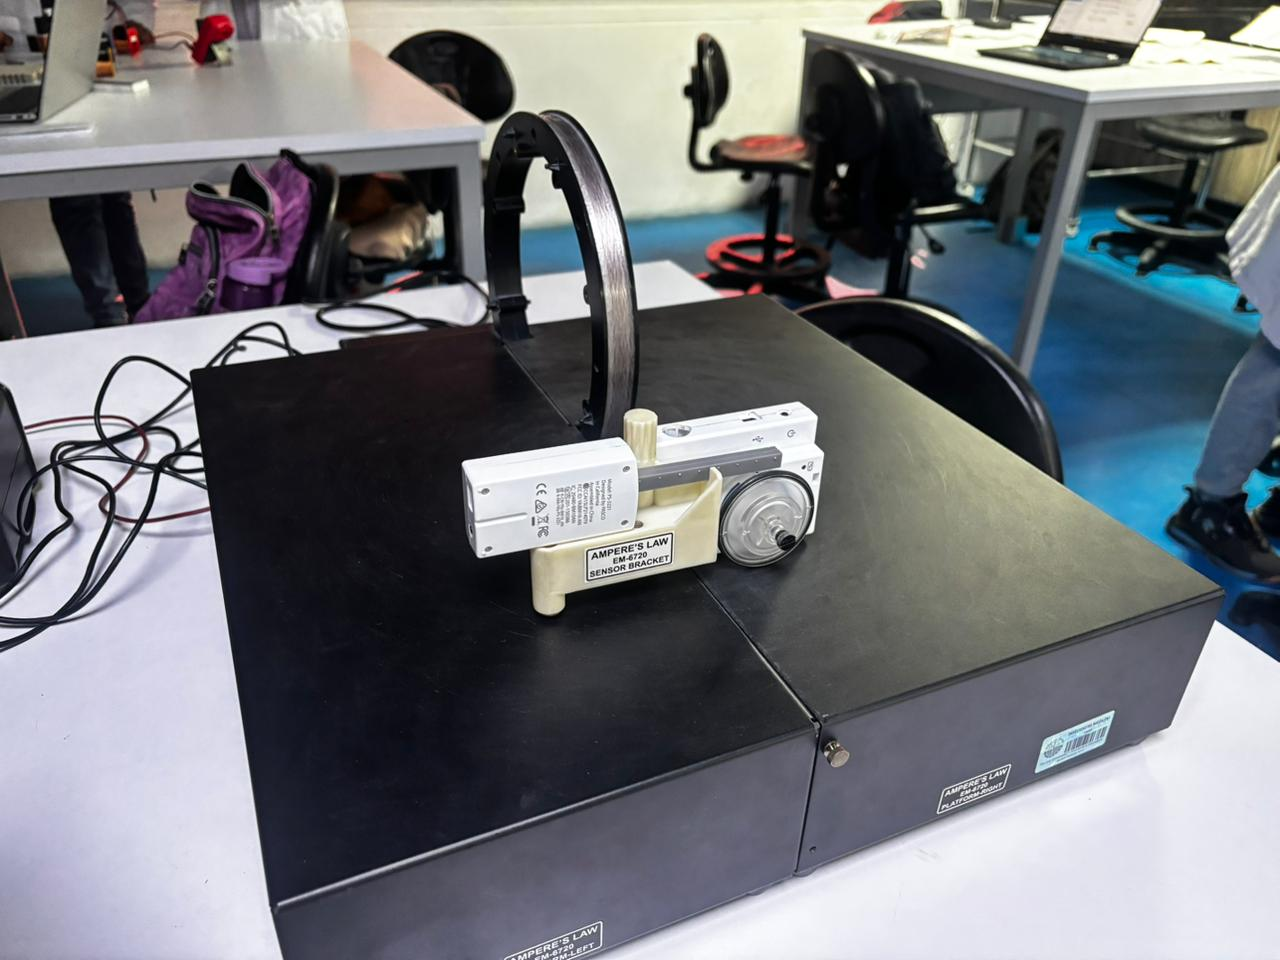
\includegraphics[width=\linewidth,height=5cm,keepaspectratio]{ampere_setup2.jpeg}
  \captionof{figure}{Aparato PASCO EM-6720: aro portador de corriente montado verticalmente y carro con sensor magnético sobre la plataforma.\label{fig:ampere_setup}}
\end{center}
\vspace{2pt}

Con $I \approx 0.815$~A y $\mu_0 NI \approx 5.12$~Gm se hicieron tres recorridos cerrados:
\begin{itemize}
    \item \textbf{Recorrido 1:} el carro pasa por el \emph{centro} del aro, enlazando la corriente.
    \item \textbf{Recorrido 2:} el carro \emph{rodea el exterior} del aro completo sin pasar por el centro.
    \item \textbf{Recorrido 3:} el carro recorre solo \emph{un lado} del aro.
\end{itemize}

\subsection*{Mesa 3: Corrientes de Foucault}

Se colgaron tres láminas planas de aluminio de una barra horizontal para que oscilaran como péndulos. Justo debajo, dos imanes permanentes con un espacio entre sus polos hacían que las láminas pasaran entre ellos al balancearse. Las tres láminas tienen geometrías distintas:
\begin{enumerate}
    \item \textbf{Lámina sólida}: sin cortes, superficie continua.
    \item \textbf{Lámina con orificios cerrados}: recortes rectangulares que no llegan a ningún borde.
    \item \textbf{Lámina tipo peine}: ranuras finas y densas abiertas en el borde inferior, formando ``dientes'' separados en la parte baja pero unidos por un puente sólido en la parte superior.
\end{enumerate}

\vspace{3pt}
\begin{center}
  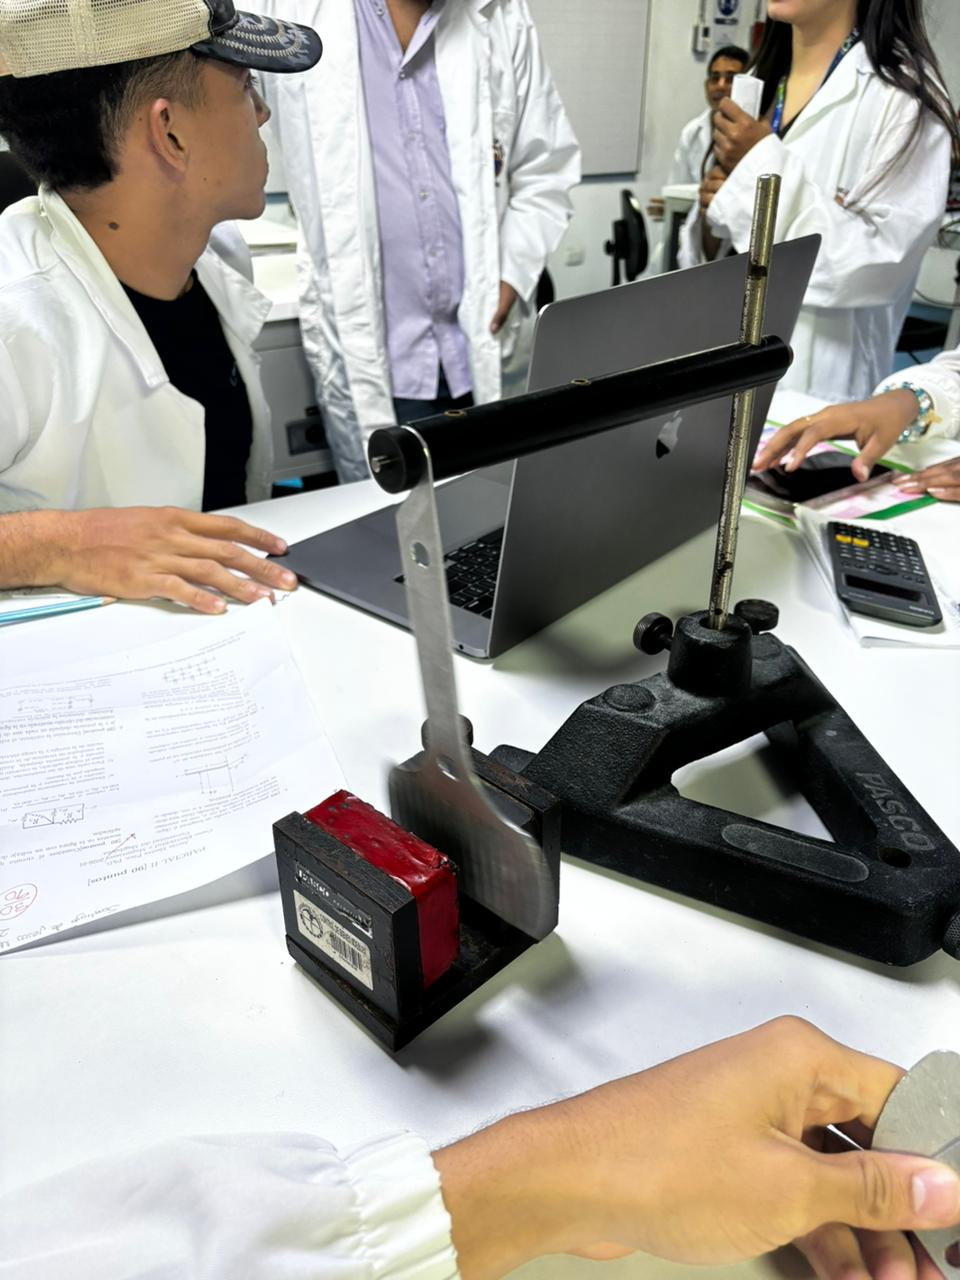
\includegraphics[width=\linewidth,height=5cm,keepaspectratio]{foucault_setup.jpeg}
  \captionof{figure}{Montaje de corrientes de Foucault: lámina de aluminio oscilando entre los polos de dos imanes permanentes.\label{fig:foucault_setup}}
\end{center}
\vspace{2pt}

\vspace{3pt}
\begin{center}
  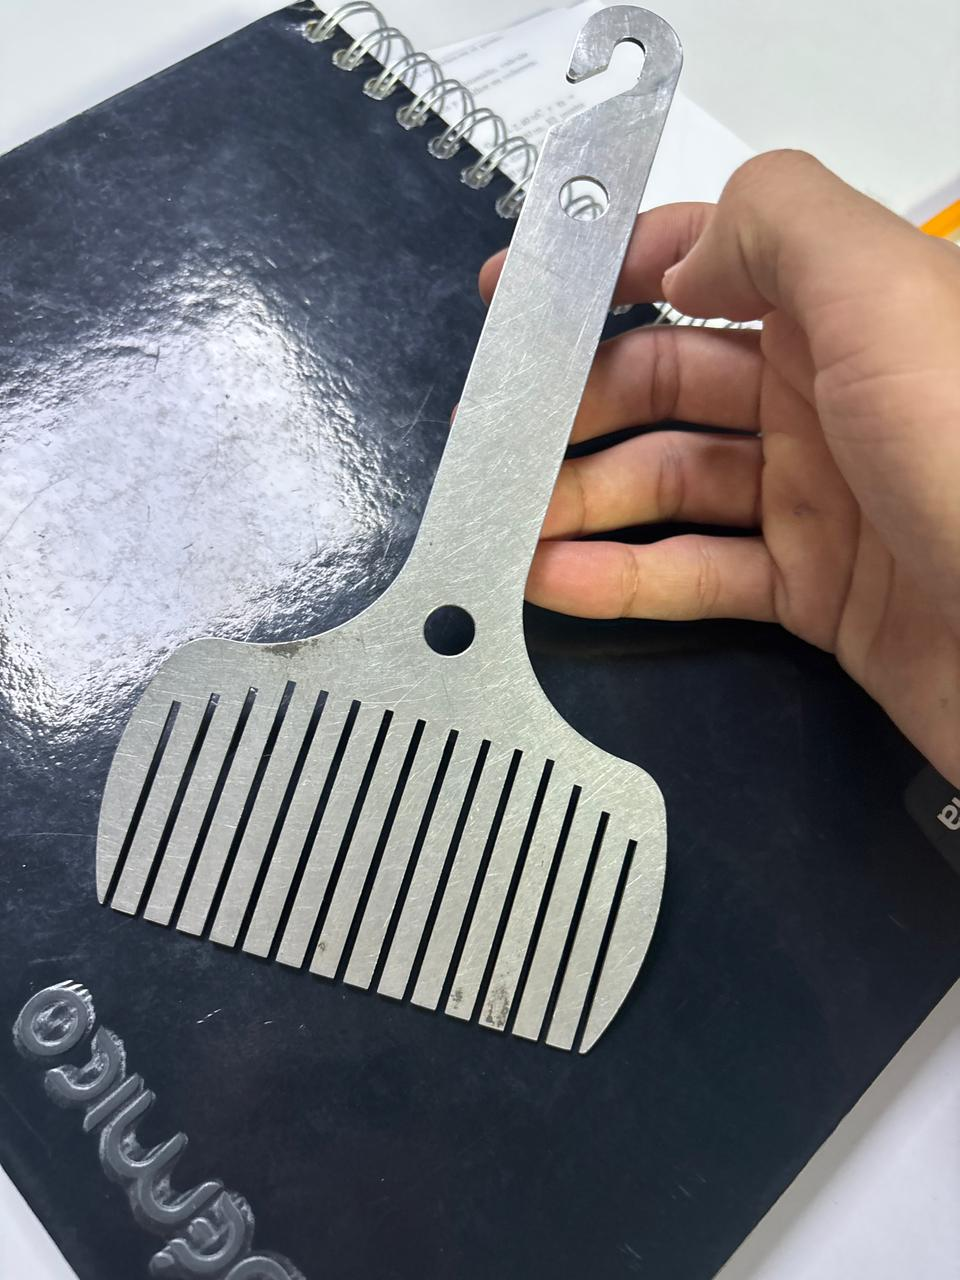
\includegraphics[width=\linewidth,height=5cm,keepaspectratio]{foucault_peine.jpeg}
  \captionof{figure}{Lámina tipo peine. Las ranuras están abiertas en el borde inferior (los dientes), pero la parte superior es un puente sólido que conecta todos los dientes.\label{fig:peine}}
\end{center}
\vspace{2pt}

\subsection*{Mesa 4: Transformador e inducción con imán}

Se usaron bobinas intercambiables Frederiksen (200, 400, 800, 1600 y 3200~espiras) con un núcleo de hierro en U y una pieza de cierre (yugo). La bobina primaria se conectó a una fuente AC de $5$~V y la secundaria a un multímetro UNI-T en modo voltaje AC.

Se probaron cuatro combinaciones de bobinas midiendo el voltaje en el secundario. Luego se desconectó el núcleo, se conectó una sola bobina al voltímetro y se pasó un imán (primero delgado, luego grande) a través de ella varias veces, registrando la fem máxima para bobinas de 200, 400 y 3200~espiras.

\vspace{3pt}
\begin{center}
  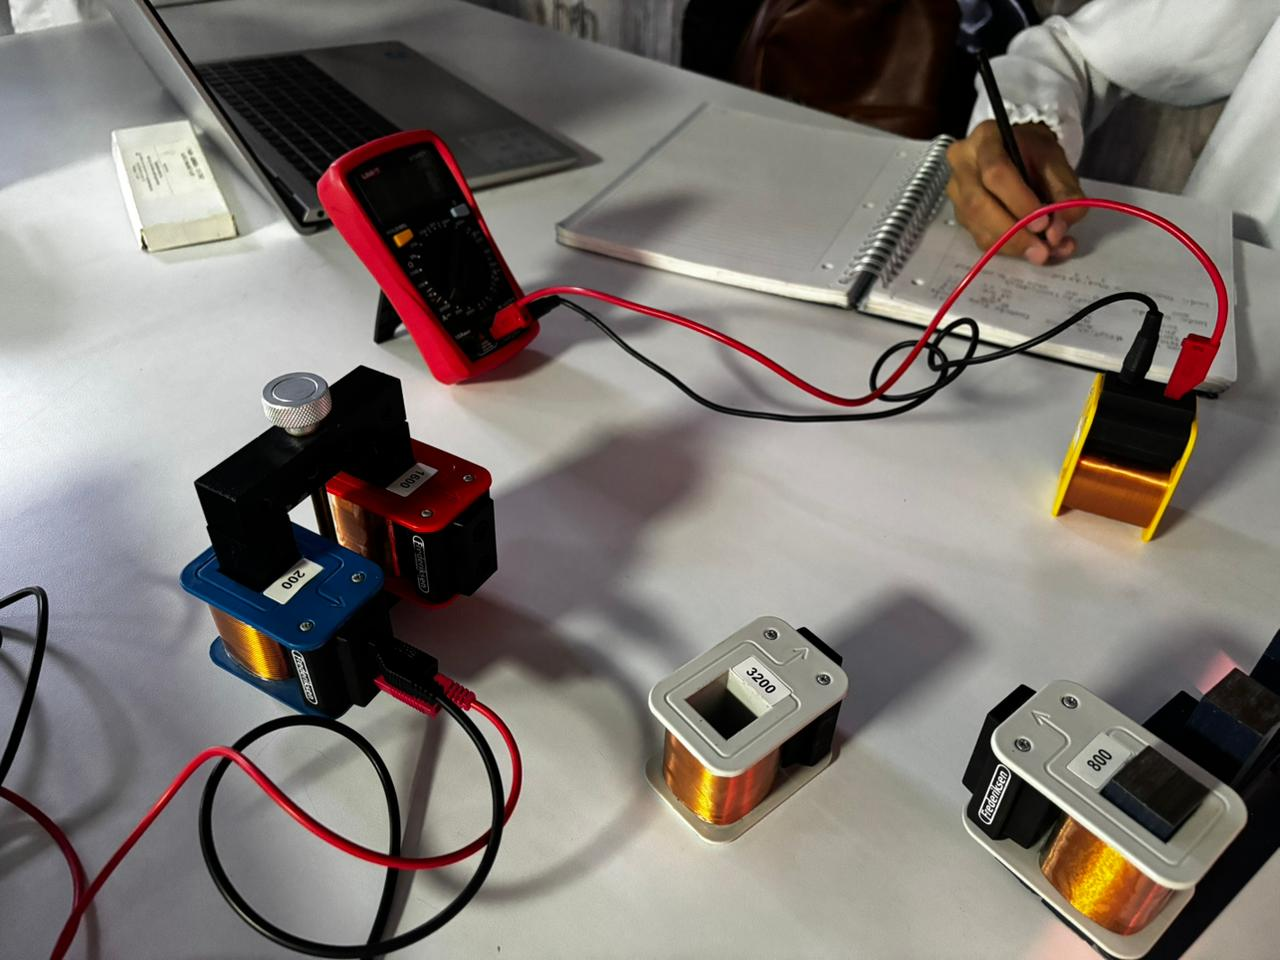
\includegraphics[width=\linewidth,height=4.5cm,keepaspectratio]{transformador.jpeg}
  \captionof{figure}{Mesa 4: bobinas Frederiksen (200 en azul, 1600 en rojo), núcleo de hierro en U con yugo y multímetro UNI-T.\label{fig:transformador}}
\end{center}
\vspace{2pt}

% -----------------------------------------------------------
\section{Resultados}
% -----------------------------------------------------------

\subsection*{Mesa 1}

La limadura se alineó de inmediato al encender la fuente. En el toroide, las líneas quedaron completamente dentro del núcleo (Fig.~\ref{fig:toroide}). En el solenoide se formaron líneas axiales densas que emergían por los extremos (Fig.~\ref{fig:solenoide}). El imán cilíndrico en la cápsula 3D mostró el patrón dipolar clásico: líneas saliendo de un polo y cerrándose en el otro.

\subsection*{Mesa 2 – Ley de Ampere}

Los resultados de cada recorrido se muestran en la Tabla~\ref{tab:ampere}.

\vspace{2pt}
\begin{center}
\captionof{table}{Integral de línea en los tres recorridos. $I = 0.815$~A, $\mu_0 NI = 5.12$~Gm.\label{tab:ampere}}
\vspace{2pt}
\small
\begin{tabular}{lcc}
\toprule
\textbf{Trayectoria} & \textbf{Área (G·m)} & \textbf{Enlaza $I$?}\\
\midrule
Por el centro  & 5.55  & Sí \\
Rodea exterior & 0.933 & No \\
Solo un lado   & 0.263 & No \\
\bottomrule
\end{tabular}
\end{center}
\vspace{2pt}

\vspace{3pt}
\begin{center}
  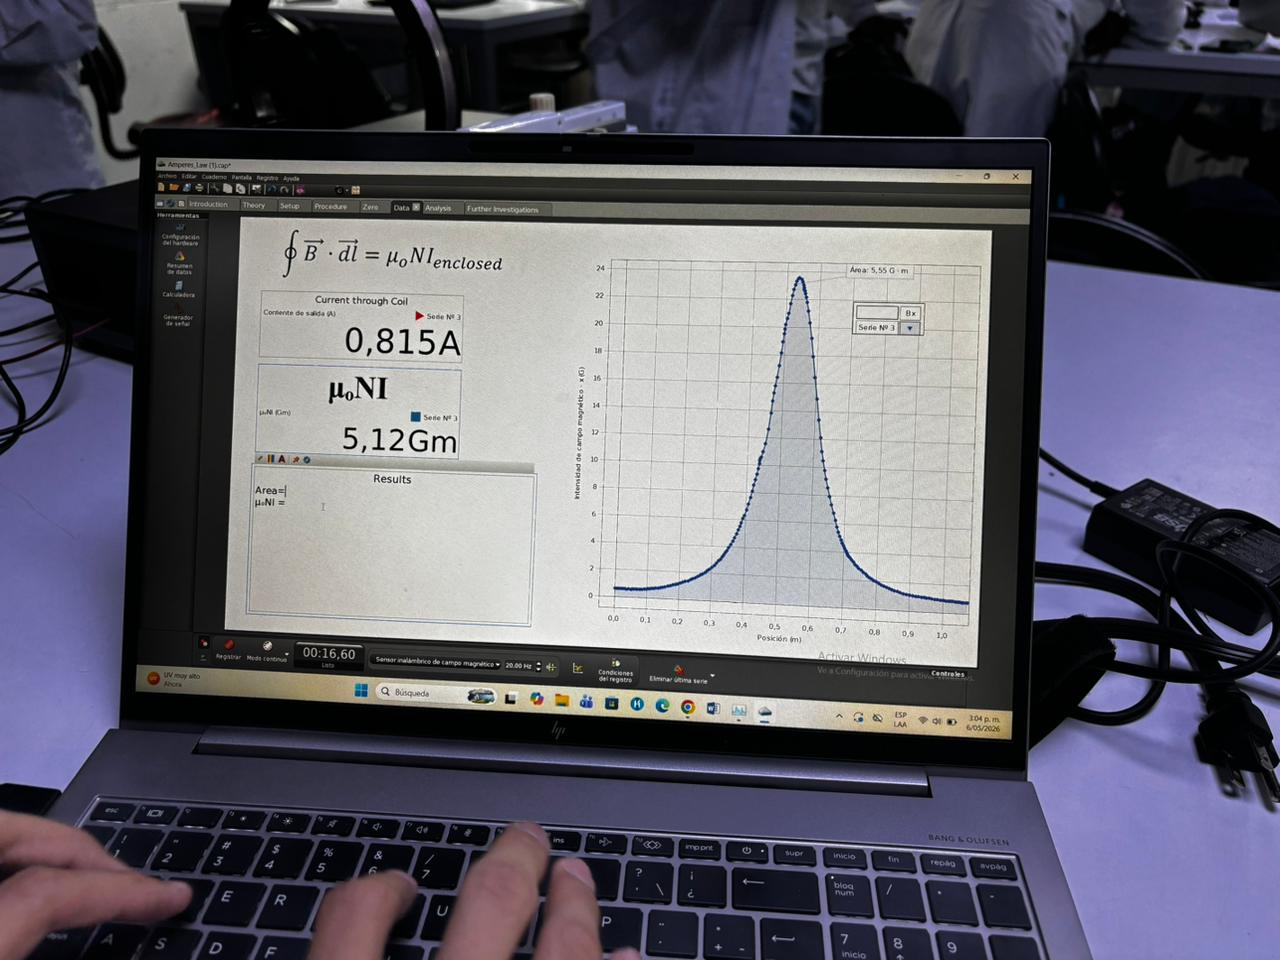
\includegraphics[width=\linewidth,height=4.5cm,keepaspectratio]{ampere_g1.jpeg}
  \captionof{figure}{Recorrido 1 (por el centro): pico tipo campana, área $= 5.55$~G·m $\approx\mu_0 NI = 5.12$~Gm. $I=0.815$~A.\label{fig:ampere1}}
\end{center}
\vspace{2pt}

\vspace{3pt}
\begin{center}
  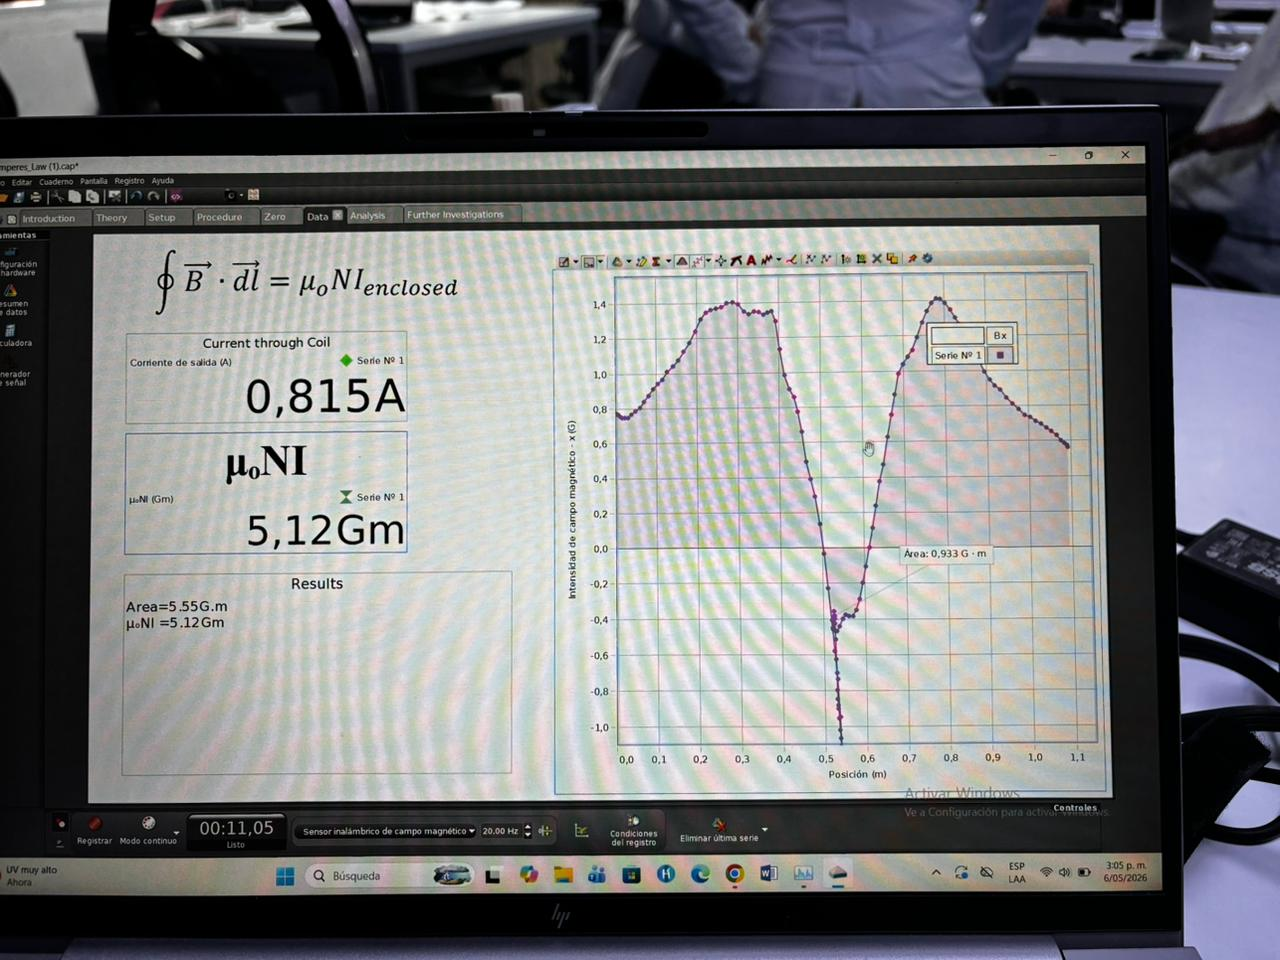
\includegraphics[width=\linewidth,height=4.5cm,keepaspectratio]{ampere_g2.jpeg}
  \captionof{figure}{Recorrido 2 (rodea el exterior): regiones positivas y negativas que casi se cancelan; área $= 0.933$~G·m $\approx 0$.\label{fig:ampere2}}
\end{center}
\vspace{2pt}

\vspace{3pt}
\begin{center}
  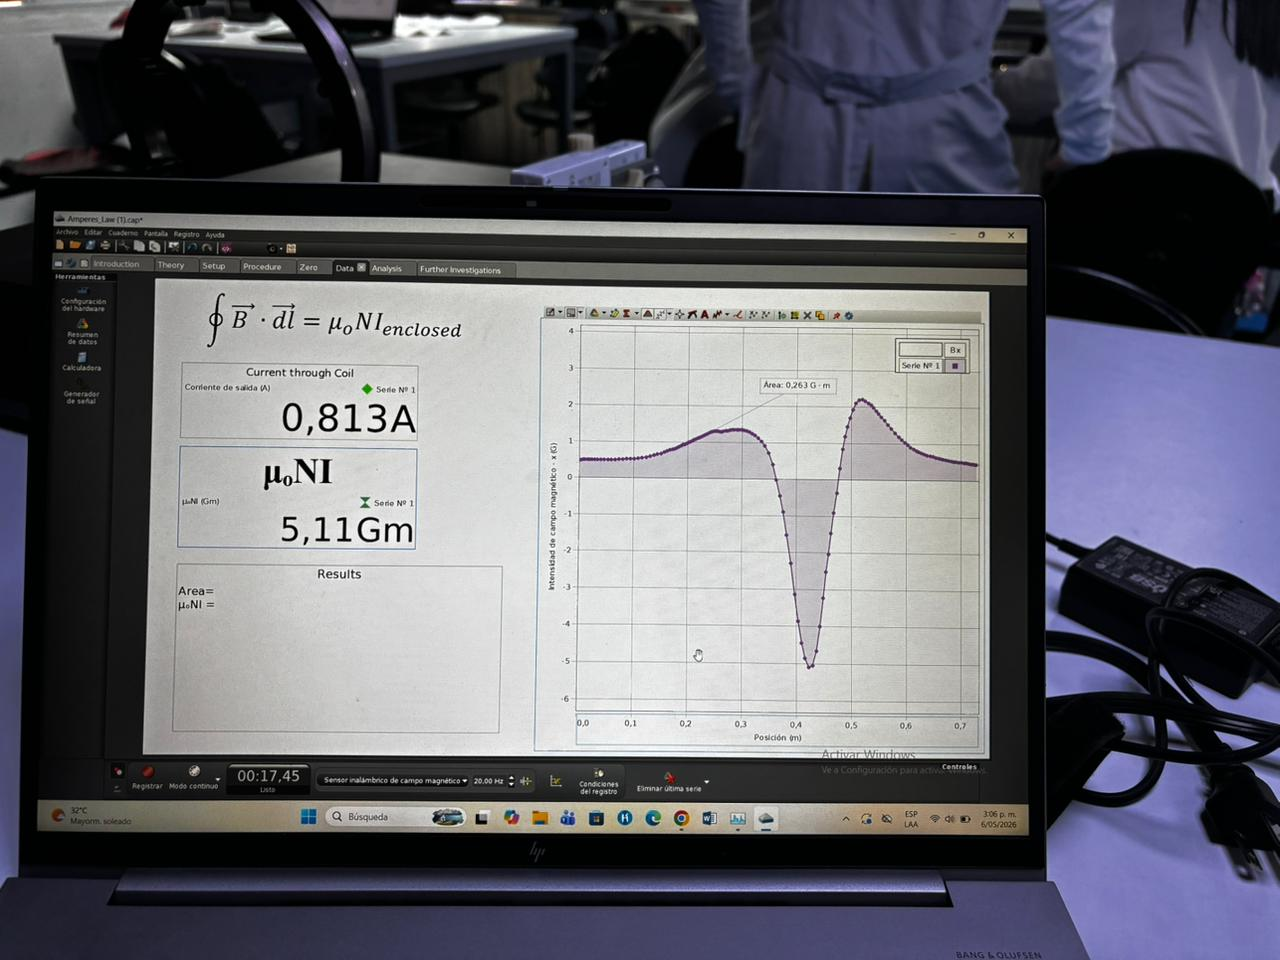
\includegraphics[width=\linewidth,height=4.5cm,keepaspectratio]{ampere_g3.jpeg}
  \captionof{figure}{Recorrido 3 (solo un lado): área $= 0.263$~G·m $\approx 0$. $I=0.813$~A.\label{fig:ampere3}}
\end{center}
\vspace{2pt}

\subsection*{Mesa 3 – Corrientes de Foucault}

Al soltar las tres láminas con la misma amplitud inicial:
\begin{itemize}
    \item \textbf{Lámina sólida y con orificios cerrados}: se frenaron notoriamente al pasar entre los imanes, deteniéndose casi por completo.
    \item \textbf{Lámina tipo peine} (señalada con flechas rojas en Fig.~\ref{fig:placas}): se detuvo completamente y de forma muy abrupta, incluso más que las otras dos.
\end{itemize}

\vspace{3pt}
\begin{center}
  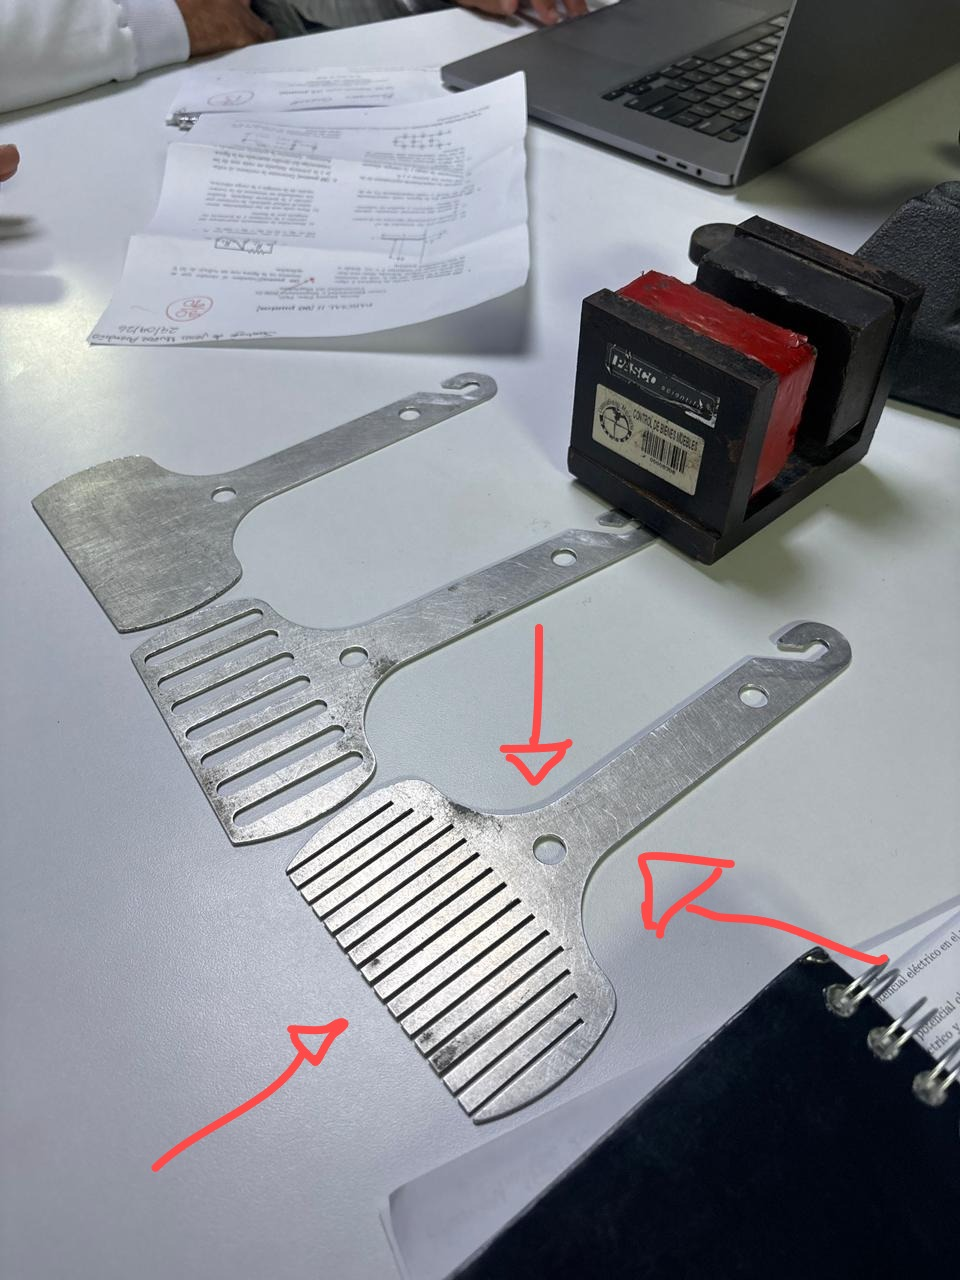
\includegraphics[width=\linewidth,height=5.5cm,keepaspectratio]{foucault_placas.jpeg}
  \captionof{figure}{Las tres láminas del experimento. Las flechas rojas señalan la lámina tipo peine (centro), que presentó el mayor frenado.\label{fig:placas}}
\end{center}
\vspace{2pt}

\subsection*{Mesa 4 – Transformador e inducción}

\textbf{Transformador:} La Tabla~\ref{tab:transformador} compara los voltajes teóricos y medidos.

\vspace{2pt}
\begin{center}
\captionof{table}{Resultados del transformador ($V_p = 5$~V AC).\label{tab:transformador}}
\vspace{2pt}
\small
\begin{tabular}{ccccr}
\toprule
$N_p$ & $N_s$ & $V_s^{\text{teór.}}$ & $V_s^{\text{med.}}$ & Efic.\\
\midrule
1600 & 3200 & 10.0~V & 8.2~V  & 82\,\%\\
1600 & 400  & 1.25~V & 1.0~V  & 80\,\%\\
200  & 3200 & 80.0~V & 31.3~V & 39\,\%\\
200  & 1600 & 40.0~V & 35.4~V & 89\,\%\\
\bottomrule
\end{tabular}
\end{center}
\vspace{2pt}

\textbf{Inducción con imán:} La Tabla~\ref{tab:faraday} resume los rangos de fem medidos.

\vspace{2pt}
\begin{center}
\captionof{table}{fem inducida al mover los imanes. Los valores dependen de la velocidad de paso.\label{tab:faraday}}
\vspace{2pt}
\small
\begin{tabular}{lcc}
\toprule
\textbf{Bobina} & \textbf{Imán delgado} & \textbf{Imán grande}\\
\midrule
200 espiras  & 0 -- 29.7~mV & 0 -- 3.4~mV \\
400 espiras  & 0 -- 30~mV   & 1 -- 7.4~mV \\
3200 espiras & 0 -- 4.8~V   & 0 -- 83~mV  \\
\bottomrule
\end{tabular}
\end{center}
\vspace{2pt}

% -----------------------------------------------------------
\section{Análisis}
% -----------------------------------------------------------

\subsection*{Mesa 1}

Los resultados confirman lo que dice la teoría. En el \textbf{toroide}, el campo queda totalmente encerrado en su interior, lo que explica por qué esa forma geométrica se usa en electrónica cuando se quiere evitar que el campo magnético interfiera con otros componentes. En el \textbf{solenoide}, las líneas en el interior son paralelas y uniformes y se cierran por los extremos, igual que en un imán de barra, lo cual justifica el nombre de ``electroimán'' cuando se le pone un núcleo de hierro. El \textbf{imán cilíndrico} en la cápsula 3D deja claro que los diagramas de campo en papel son solo un corte de algo que ocurre en todas las direcciones del espacio.

\subsection*{Mesa 2 – Ley de Ampere}

Para el Recorrido~1 (pasa por el centro), el área medida fue $5.55$~G·m frente al valor teórico $\mu_0 NI = 5.12$~Gm, lo que da un error de:
\begin{equation}
    \varepsilon_1 = \frac{|5.55 - 5.12|}{5.12}\times 100\% \approx 8.4\,\%.
\end{equation}
Este error es razonablemente pequeño. Se debe principalmente a que el carro no traza un camino perfectamente cerrado (el inicio y el final no coinciden con exactitud), a pequeñas vibraciones del sensor durante el desplazamiento y a posibles interferencias de otros equipos en el laboratorio.

Para los Recorridos~2 y~3, que no enlazan la corriente, la integral debería ser cero. Los valores obtenidos fueron $0.933$~G·m y $0.263$~G·m, respectivamente, lo que como porcentaje del valor de referencia equivale a errores del $\approx18\,\%$ y $\approx5\,\%$. Estos residuos se atribuyen a las mismas fuentes: el camino no cierra perfectamente y el sensor acumula pequeñas derivas.

El resultado más importante es la diferencia en magnitud: la Trayectoria~1 dio $5.55$~G·m mientras que las otras dos dieron valores más de diez veces menores. Esto confirma el principio central de la ley de Ampere: \emph{lo que determina el valor de la integral no es la forma del camino, sino si ese camino encierra o no la corriente}. Cuando el camino pasa por el centro del aro y enlaza la corriente, la integral es aproximadamente $\mu_0 NI$; cuando no la encierra, sin importar cómo rodee el aro por fuera, la integral es prácticamente cero.

\subsection*{Mesa 3 – Corrientes de Foucault}

Lo que determina cuánto se frena cada lámina es si hay caminos cerrados disponibles para que las corrientes puedan circular.

La \textbf{lámina sólida} no tiene ninguna interrupción, así que los electrones pueden describir lazos grandes que encierran mucho flujo magnético. Eso genera corrientes grandes que, por la ley de Lenz, frenan la lámina con mucha fuerza.

La \textbf{lámina tipo peine} es el caso más interesante. Tiene las ranuras abiertas en el borde inferior (los dientes), pero la parte de arriba es un \textbf{puente sólido continuo} que conecta todos los dientes. Cuando la lámina pasa entre los imanes, las corrientes pueden circular siguiendo un recorrido en forma de U invertida: suben por un diente, cruzan el puente superior y bajan por el diente de al lado. Este lazo encierra prácticamente la misma área que en una lámina sólida, así que la fem inducida es igual de grande y el frenado es igual de intenso. Por eso esta lámina se detiene de forma tan abrupta.

La clave está en que \emph{no basta con hacer cortes en un conductor para eliminar las corrientes de Foucault}. Los cortes deben romper completamente todos los lazos posibles de corriente. Si queda un puente sólido conectando las tiras, la corriente sigue encontrando camino. Este es exactamente el motivo por el que los núcleos de los transformadores se fabrican con láminas delgadas separadas por capas aislantes [3].

\subsection*{Mesa 4 – Transformador e inducción}

\textbf{Transformador:} Para los primarios de 1600 espiras, la eficiencia fue del $80$--$82\,\%$, lo cual es coherente con las pérdidas normales de un transformador de laboratorio: resistencia del alambre, histéresis en el núcleo y un poco de flujo que no llega al secundario.

El caso más llamativo es el \textbf{primario de 200 espiras con secundario de 3200} (fila~3 de la Tabla~\ref{tab:transformador}): medimos $31.3$~V en lugar de los $80$~V teóricos, lo que da apenas un $39\,\%$ de eficiencia. Esto ocurre porque con tan pocas espiras en el primario, su inductancia es muy baja (la inductancia crece con $N_p^2$, así que pasar de 1600 a 200 espiras la reduce 64 veces). Una inductancia baja significa que el primario se comporta más como una resistencia que como una bobina, y gran parte de la energía se disipa en calor en lugar de transferirse al secundario. En cambio, el caso \textbf{200/1600} (fila~4) funciona mejor ($89\,\%$) porque la relación de transformación es menor y las pérdidas no se amplifican tanto.

\textbf{Inducción con imán:} Los datos de la Tabla~\ref{tab:faraday} muestran que la fem crece con el número de espiras, en línea con la ley de Faraday. Para el imán grande, la proporcionalidad es bastante clara:
\begin{align*}
    \frac{\mathcal{E}_{400}}{\mathcal{E}_{200}} &= \frac{7.4}{3.4} \approx 2.2 \approx \frac{400}{200} = 2\quad(\checkmark),\\
    \frac{\mathcal{E}_{3200}}{\mathcal{E}_{200}} &= \frac{83}{3.4} \approx 24 \;\gtrsim\; \frac{3200}{200} = 16.
\end{align*}
La razón 3200/200 medida ($\approx24$) es algo mayor que el factor teórico (16), lo que se explica porque en ese ensayo el imán probablemente se movió más rápido (mayor $d\Phi_B/dt$), amplificando la fem. Esto es consistente con la anotación del cuaderno: ``varía con la velocidad''.

Para el imán delgado, los valores de 200 y 400 espiras son casi iguales ($\approx 30$~mV), lo que indica que en ambos casos el imán se pasó a velocidades muy similares. El salto a $4.8$~V para 3200 espiras (un factor $\approx160$ en lugar del factor 8 esperado solo por las espiras) confirma que ese ensayo se realizó con mucha mayor velocidad. El hecho de que el imán delgado produzca una fem mayor que el grande a igual bobina también puede explicarse porque fue manipulado con mayor velocidad, o porque al ser más delgado concentra mejor el flujo en el área de la bobina.

En conjunto, los resultados verifican cuantitativamente que $\mathcal{E} \propto N$ y que la velocidad del imán tiene un efecto directo sobre la magnitud de la fem inducida.

% -----------------------------------------------------------
\section{Conclusiones}
% -----------------------------------------------------------

Los cuatro experimentos permitieron verificar de forma directa los principios fundamentales del electromagnetismo clásico.

La visualización con limadura de hierro demostró que las líneas de campo son lazos cerrados cuya geometría depende de la configuración del conductor o imán: el toroide las confina, el solenoide las proyecta axialmente y el imán cilíndrico las distribuye en forma dipolar en tres dimensiones.

La verificación de la ley de Ampere confirmó su carácter topológico: cuando el camino encierra la corriente, la integral vale $\approx\mu_0 NI$ (error de $8.4\,\%$); cuando no la encierra, el resultado es prácticamente cero. La forma del camino no importa, solo importa si encierra o no la corriente.

En las corrientes de Foucault se comprobó que la geometría de las ranuras es determinante. La lámina tipo peine se frenó completamente porque su puente sólido superior permite que las corrientes formen lazos grandes entre los dientes. Esto muestra que los cortes solo reducen el frenado si interrumpen \emph{completamente} todos los lazos de corriente posibles.

Finalmente, el transformador confirmó la relación $V_s/V_p = N_s/N_p$ con eficiencias del $80$--$89\,\%$ para primarios de 1600 espiras, pero con solo $39\,\%$ para el primario de 200 espiras, evidenciando que la inductancia del primario es clave para un buen desempeño. El experimento de inducción con imán verificó que $\mathcal{E} \propto N$ y que la velocidad del imán afecta directamente la fem inducida.

% -----------------------------------------------------------
\section{Referencias}
% -----------------------------------------------------------

\noindent [1] D. J. Griffiths, \textit{Introduction to Electrodynamics}, 4.ª~ed., Cambridge University Press (2017).

\noindent [2] P. A. Tipler y G. Mosca, \textit{Física para la Ciencia y la Tecnología}, vol.~2, 6.ª~ed., Reverté (2010).

\noindent [3] H. D. Young y R. A. Freedman, \textit{Sears-Zemansky Física Universitaria}, vol.~2, 14.ª~ed., Pearson (2018).

\noindent [4] PASCO Scientific, \textit{Ampere's Law Apparatus EM-6720 Instruction Manual}, PASCO (2019).

\noindent [5] Frederiksen, \textit{Transformer Coils 2855.00 User Guide}, Frederiksen (2015).

\end{multicols}
\end{document}
